\chapter{STRUKTUR DATA / BASIS DATA}

Karena pencatatan pembayaran dari Bank Kas Daerah tercatat pada sistem informasi atau aplikasi SISMIOP (Sistem Manajemen Informasi Objek Pajak), maka struktur basis data yang digunakan pada sistem informasi pembayaran Pajak Bumi dan Bangunan sektor Perdesaan dan Perkotaan menggunakan beberapa tabel pada aplikasi SISMIOP (Sistem Manajemen Informasi Objek Pajak). Tabel-tabel yang digunakan adalah seperti berikut ini :

\section{Tabel SPPT}

Tabel ini selain mencatatkan ketetapan untuk tiap objek pajak pada tiap tahun pajak, tabel ini juga mencatatkan status pembayaran apakah sudah lunas atau belum. Struktur tabelnya adalah seperti pada gambar \ref{fig:struktur-sppt} berikut ini :

\begin{figure}[H]
	\centering
	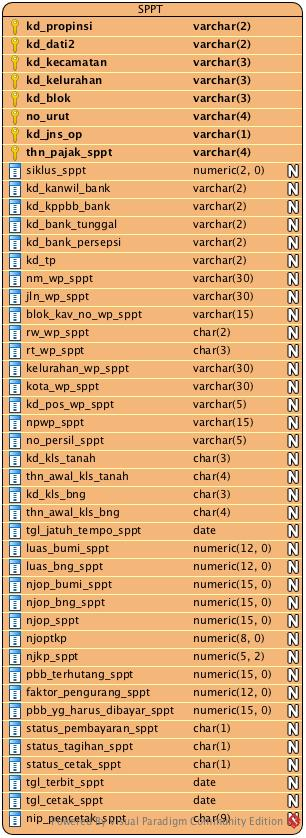
\includegraphics[width=0.5\textwidth]{./resources/struktur-tabel-sppt}
	\caption{Struktur Tabel \texttt{SPPT}}
	\label{fig:struktur-sppt}
\end{figure}

Dari struktur tabel \texttt{SPPT} di atas, beberapa \textit{field} atau kolom yang digunakan pada sistem informasi atau aplikasi ini adalah seperti berikut :

\begin{itemize}
	\item Nomor Objek Pajak, yang terdiri dari \textit{field} atau kolom \texttt{kd\_propinsi}, \texttt{kd\_dati2}, \texttt{kd\_kecamatan}, \texttt{kd\_kelurahan}, \texttt{kd\_blok}, \texttt{no\_urut}, dan \texttt{kd\_jns\_op}.
	\item Tahun pajak pada \textit{field} atau kolom \texttt{thn\_pajak\_sppt}.
	\item Nama wajib pajak pada \textit{field} atau kolom \texttt{nm\_wp\_sppt}
	\item Besarnya pajak terhutang pada \textit{field} atau kolom \texttt{pbb\_yg\_harus\_dibayar\_sppt}
	\item Status pembayaran pada \textit{field} atau kolom \texttt{status\_pembayaran\_sppt}
\end{itemize}

\section{Tabel DAT\_OBJEK\_PAJAK}

Tabel \texttt{DAT\_OBJEK\_PAJAK}, digunakan untuk menampilkan informasi mengenai objek pajak seperti alamat, luas bumi dan bangunan, serta Nilai Jual Objek Bumi dan Bangunan. Struktur tabel dari \texttt{DAT\_OBJEK\_PAJAK} adalah seperti pada gambar \ref{fig:struktur-dat-op} berikut ini :

\begin{figure}[H]
	\centering
	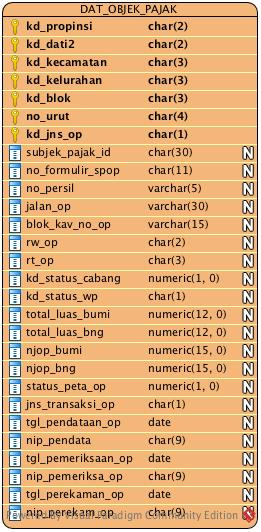
\includegraphics[width=0.5\textwidth]{./resources/struktur-tabel-dat-op}
	\caption{Struktur Tabel \texttt{DAT\_OBJEK\_PAJAK}}
	\label{fig:struktur-dat-op}
\end{figure}

Informasi yang digunakan pada tabel \texttt{DAT\_OBJEK\_PAJAK} ini ada di beberapa \textit{field} atau kolom seperti berikut :

\begin{itemize}
	\item Alamat, akan menggunakan gabungan dari \textit{field} atau kolom \texttt{jalan\_op}, \texttt{blok\_kav\_no\_op}, \texttt{rw\_op}, dan \texttt{rt\_op}.
	\item Luas bumi akan menggunakan \textit{field} atau kolom \texttt{total\_luas\_bumi}.
	\item Luas bangunan akan menggunakan \textit{field} atau kolom \texttt{total\_luas\_bng}.
	\item Nilai Jual Objek Pajak (NJOP) bumi akan menggunakan \textit{field} atau kolom \texttt{njop\_bumi}.
	\item Nilai Jual Objek Pajak (NJOP) bangunan akan menggunakan \textit{field} atau kolom \texttt{njop\_bng}.
\end{itemize}

\section{Tabel DAT\_SUBJEK\_PAJAK}

Tabel \texttt{DAT\_SUBJEK\_PAJAK} ini digunakan untuk menampilkan informasi mengenai subjek pajak seperti nama dan alamatnya. Struktur tabel dari \texttt{DAT\_SUBJEK\_PAJAK} ini adalah seperti pada gambar \ref{fig:struktur-dat-sp} berikut ini :

\begin{figure}[H]
	\centering
	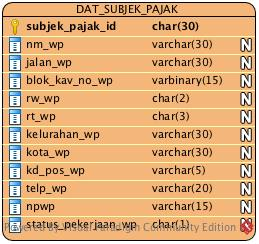
\includegraphics[width=0.5\textwidth]{./resources/struktur-tabel-dat-sp}
	\caption{Struktur Tabel \texttt{DAT\_SUBJEK\_PAJAK}}
	\label{fig:struktur-dat-sp}
\end{figure}

Informasi pada tabel \texttt{DAT\_SUBJEK\_PAJAK} yang digunakan ada pada beberapa \textit{field} atau kolom berikut :

\begin{itemize}
	\item Nama subjek pajak pada \textit{field} atau kolom \texttt{nm\_wp}
	\item Alamat subjek pajak pada \textit{field} atau kolom \texttt{jalan\_wp}, \texttt{blok\_kav\_no\_wp}, \texttt{rw\_wp}, \texttt{rt\_wp}, \texttt{kelurahan\_wp}, dan \texttt{kota\_wp}.
\end{itemize}

\section{Tabel REF\_KECAMATAN}

Untuk tabel \texttt{REF\_KECAMATAN} digunakan hanya untuk menampilkan informasi nama Kecamatan dimana objek berada. Struktur tabel untuk \texttt{REF\_KECAMATAN} ini seperti terlihat pada gambar \ref{fig:struktur-ref-kec} berikut ini :

\begin{figure}[H]
	\centering
	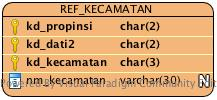
\includegraphics[width=0.5\textwidth]{./resources/struktur-tabel-ref-kec}
	\label{fig:struktur-ref-kec}
	\caption{Struktur Tabel \texttt{REF\_KECAMATAN}}
\end{figure}

Informasi yang digunakan pada tabel \texttt{REF\_KECAMATAN} ini ada pada beberapa \textit{field} atau kolom seperti berikut ini :

\begin{itemize}
	\item Nomor Identifikasi Kecamatan, pada \textit{field} atau kolom \texttt{kd\_propinsi}, \texttt{kd\_dati2}, dan \texttt{kd\_kecamatan}
	\item Nama Kecamatan, pada \textit{field} atau kolom \texttt{nm\_kecamatan}.
\end{itemize}

\section{Tabel REF\_KELURAHAN}

Tabel \texttt{REF\_KELURAHAN} pun digunakan hanya untuk menampilkan nama Kelurahan / Desa dimana objek pajak berada. Struktur tabel \texttt{REF\_KELURAHAN} ini seperti terlihat pada gambar \ref{fig:struktur-ref-kel} berikut ini :

\begin{figure}[H]
	\centering
	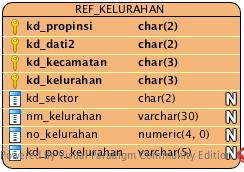
\includegraphics[width=0.5\textwidth]{./resources/struktur-tabel-ref-kel}
	\caption{Struktur Tabel \texttt{REF\_KELURAHAN}}
	\label{fig:struktur-ref-kel}
\end{figure}

Informasi pada tabel \texttt{REF\_KELURAHAN} yang digunakan ada pada beberapa \textit{field} atau kolom berikut ini :

\begin{itemize}
	\item Nomor Identifikasi Kelurahan / Desa pada \textit{field} atau kolom \texttt{kd\_propinsi}, \texttt{kd\_dati2}, \texttt{kd\_kecamatan}, dan \texttt{kd\_kelurahan}.
	\item Nama Desa / Kelurahan pada \textit{field} atau kolom \texttt{nm\_kelurahan}
\end{itemize}